\documentclass[twoside,twocolumn]{article}
\usepackage{amsmath}
\usepackage{amsfonts}
\usepackage{amssymb}
\usepackage{graphicx}
\usepackage{blindtext} % Package to generate dummy text throughout this template 

\usepackage[hmarginratio=1:1,top=32mm,columnsep=20pt]{geometry} % Document margins
\usepackage[hang, small,labelfont=bf,up,textfont=it,up]{caption} % Custom captions under/above floats in tables or figures
\usepackage{booktabs} % Horizontal rules in tables
\usepackage{lettrine} % The lettrine is the first enlarged letter at the beginning of the text

\usepackage{enumitem} % Customized lists
\setlist[itemize]{noitemsep} % Make itemize lists more compact

\usepackage{abstract} % Allows abstract customization
\renewcommand{\abstractnamefont}{\normalfont\bfseries} % Set the "Abstract" text to bold
\renewcommand{\abstracttextfont}{\normalfont\small\itshape} % Set the abstract itself to small italic text

\usepackage{titlesec} % Allows customization of titles
\renewcommand\thesection{\Roman{section}} % Roman numerals for the sections
\renewcommand\thesubsection{\roman{subsection}} % roman numerals for subsections
\titleformat{\section}[block]{\large\scshape\centering}{\thesection.}{1em}{} % Change the look of the section titles
\titleformat{\subsection}[block]{\large}{\thesubsection.}{1em}{} % Change the look of the section titles

\usepackage{fancyhdr} % Headers and footers
\pagestyle{fancy} % All pages have headers and footers
\fancyhead{} % Blank out the default header
\fancyfoot{} % Blank out the default footer
\fancyhead[C]{Patrones de Diseño del Software $\bullet$ Noviembre 2020 $\bullet$ } % Custom header text
\fancyfoot[RO,LE]{\thepage} % Custom footer text

\usepackage{titling} % Customizing the title section

\usepackage{hyperref} % For hyperlinks in the PDF

%----------------------------------------------------------------------------------------
%	TITLE SECTION
%----------------------------------------------------------------------------------------

\setlength{\droptitle}{-4\baselineskip} % Move the title up

\pretitle{\begin{center}\Huge\bfseries} % Article title formatting
\posttitle{\end{center}} % Article title closing formatting
\title{Mejoramiento del Proyecto Gas} % Article title
\author{MamaniPerez Luis,Carpio Alejandro,Mamani Laura Juan,LaTorre Jose,Yanqui  Rodrigo}
\date{\today} % Leave empty to omit a date

\renewcommand{\maketitlehookd}
{%
\begin{abstract}
\noindent La implementación de un software nos permitirá entender los beneficios que se tiene al momento cuando el usuario este en la posibilidad de utilizarlo. El uso del software agiliza los procesos en cualquier tipo de organización, como las empresas, negocios, organizaciones y otras que requiera del uso de ordenadores. Este programa está diseñado en un entorno de escritorio en el lenguaje java, el programa puede contener fallas, bugs entre otros errores que al hacer las pruebas con SonarQube nos podremos dar cuenta. En este documento lo que se trata de mostrar es el proceso de mejoramiento del Sistema GAS con SonarQube. La Herramienta SonarQube permite analizar el código fuente, en diversos lenguajes, y realizar un seguimiento continuo sobre la calidad del software. 

\end{abstract}
}
%----------------------------------------------------------------------------------------

\begin{document}

% Print the title
\maketitle

%----------------------------------------------------------------------------------------
%	ARTICLE CONTENTS
%----------------------------------------------------------------------------------------

\section{Introduccion}

\lettrine[nindent=0em,lines=2]{P}ara este trabajo final de la Segunda Unidad usaremos la herramienta MongoDB para crear un . Esta herramienta nos ayudara a mejorar la calidad del Sistema Gas, que se hizo en ciclos anteriores. SonarQube nos permitirá evaluar el código fuente, con esto podremos obtener una métrica que nos pueden ayudar en la calidad del código fuente del Sistema GAS.

%------------------------------------------------
\section{Objetivos}

\begin{itemize}
\item Entender la problemática.
\item Entender la justificación del proyecto.
\item Alcance del proyecto.
\item Objetivo del proyecto.
\item Desarrollo del proyecto.

\end{itemize}
%------------------------------------------------

\section{Desarrollo}

\subsection{¿Cual es la problematica?}
El problema principal es que el programa actual cuenta con muchos problemas de código, quizás cosas que no afecten al funcionamiento del programa, pero sí a su rendimiento. Dicho esto, el código fuente actual puede ser mejorable. 
 
\subsection{¿Cuales son la justificaciones del proyecto?}

\begin{itemize}
\item[1]¿Que se va a hacer? 
\newline
\newline
Una mejora al código fuente del Sistema GAS con la herramienta SonarQube. 
\newline
\item[2]¿Por que se va a hacer? 
\newline
\newline
Porque el programa necesita una mejora en el código fuente. 
\newline
\item[3]¿Para que se va a hacer? 
\newline
\newline
Para tener un mejor rendimiento del programa, y utilizar la herramienta que aprendimos en esta unidad: SonarQube. 
\newline
\item[4]¿Cómo se va a hacer? 
\newline
\newline
Utilizando la herramienta SonarQube 
\newline
\item[5]¿Por qué es importante este trabajo de unidad? 
\newline
\newline
Porque esto nos ayudara a tener buenas prácticas al momento de desarrollar futuros proyectos y también a saber cómo encontrar fallas o vulneraciones en el código fuente del sistema y así poder mejorar el código fuente y como consecuencia mejorar el rendimiento del sistema
\newline
\end{itemize}

\subsection{¿Cual es el alcance del proyecto?}
\begin{itemize}
\item El plan de mejora no incluye funciones nuevas en el programa. 
\newline
\item El plan de mejora no incluye una nueva interfaz del programa. 
\newline
\item El plan de mejora incluye la mejora del código fuente. 
\newline
\item El plan de mejora incluye el uso de métricas para mejorar el código fuente. 
\end{itemize}

\subsection{¿Cual es el objetivo del proyecto?}
\begin{itemize}
\item[1] Objetivo General 
\newline
Mejorar el código fuente el Sistema Gas usando la herramienta SonarQube.  
\newline
\newline
\item[2] Objetivos Especificos 
\newline
\item Que el rendimiento del programa se vea incrementado gracias a la mejora del código fuente. 
\newline
\item Aprender de las métricas que utiliza la herramienta para que nuestros códigos futuros sean más limpios y reutilizables 
\end{itemize}
%--\includegraphics[width=6.5cm, height=4cm]{imagenes/Patrones creacionales/diagrama clases}
\subsection{Desarrollo de la propuesta}

Habiendo escaneado el proyecto nos da este resultado: 
\newline
\newline
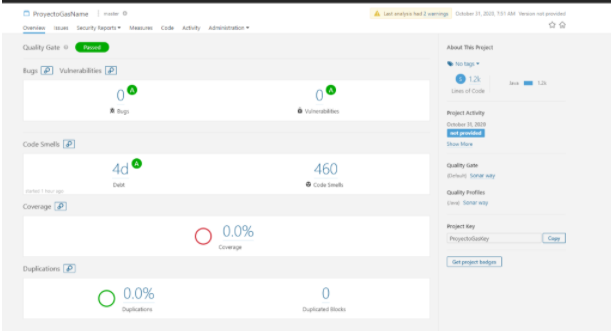
\includegraphics[width=7cm, height=5cm]{Image/1.png}
\newline
\newline
Code Smell: Es determinado como deficiencias del diseño del software. Siendo que es variado esta clase de errores, entre uso excesivo de calls y redundancia de codigo. 
\newline
\newline
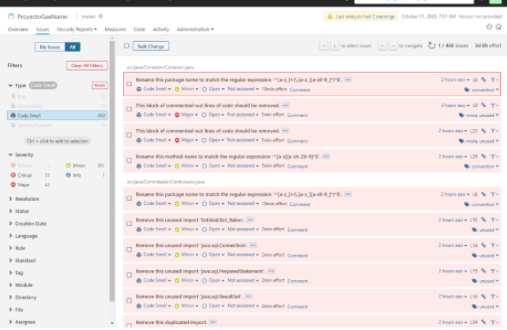
\includegraphics[width=7cm, height=5cm]{Image/2.png}
\newline
\newline
El Code Smell, no es un bug ni un error, y aunque puede no afectar de manera grave el funcionamiento del programa, suele generar retrasos en su desarrollo y hasta pueden generar problemas en el futuro. 
\newline
\newline
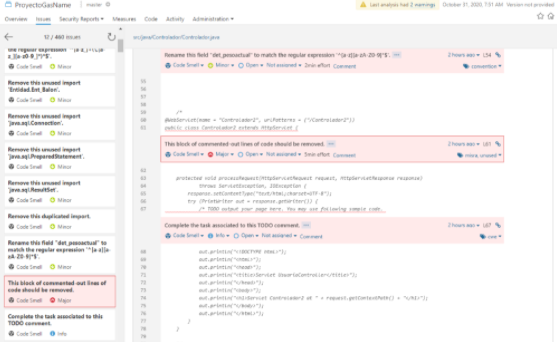
\includegraphics[width=7cm, height=5cm]{Image/3.png}
\newline
\newline
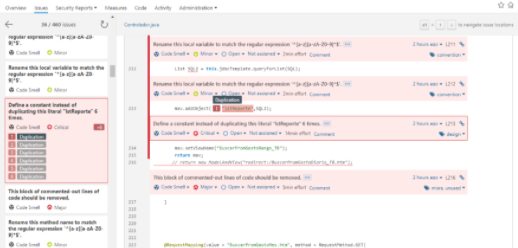
\includegraphics[width=7cm, height=5cm]{Image/4.png}
\newline
\newline
Con SonarQube es sencillo revisar a primera vista si hay un error, y la herramienta da desde consejos hasta soluciones. 
\newline
\newline
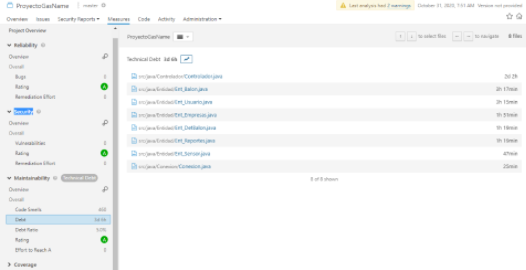
\includegraphics[width=7cm, height=5cm]{Image/5.png}
\newline
\newline
5.1 Tecnología de información 
\begin{itemize}
\item Gas
\newline
Es elemento del proyecto del cual hacemos uso para su medición y resultado
\newline
\newline
\item MYSQL
\newline
Es un sistema de gestión de base de datos (SGBD) de código abierto. El SGBD MySQL pertenece actualmente a Oracle. Funciona con un modelo cliente-servidor.  
\newline
\newline
\item JAVA
\newline
Java sirve para crear aplicaciones y procesos en una gran diversidad de dispositivos. Se base en programación orientada a objetivos, permite ejecutar un mismo programa en diversos sistemas operativos y ejecutar el código en sistemas remotos de manera segura. 
\newline
\newline
\item NETBEANS 
\newline
NetBeans es un entorno de desarrollo integrado libre, hecho principalmente para el lenguaje de programación Java. La plataforma NetBeans permite que las aplicaciones sean desarrolladas a partir de un conjunto de componentes de software llamados módulos. 
\newline
\newline
5.2 Metodología, técnicas usadas
\begin{itemize}
\item Programación Orienta a Objetos (POO) 
\newline
\newline
\item Programación en 3 Capas 
\newline
\newline
\item Marco de Trabajo de procesos agiles SCRUM 
\newline
\newline
\item Metodología RUP 
\newline
\newline
\end{itemize}
Ciclo de Vida del Proyecto 
\newline
\newline
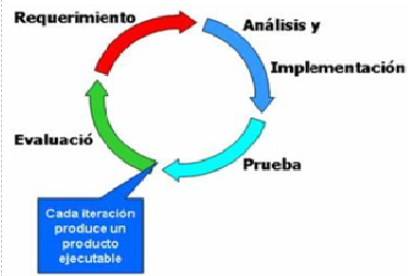
\includegraphics[width=7cm, height=5cm]{Image/6.png}

\clearpage
\section{Desarrollo de Solucion de Mejora}
Empezamos por comprender el objetivo del trabajo. Usar una base de datos Nosql, e implementar en una parte del proyecto.
Escogimos hacer un ejemplo de operaciones, conexion y ejecucion.
\subsection{Casos de Uso de la Aplicacion}

\begin{figure}[h!]
\centering
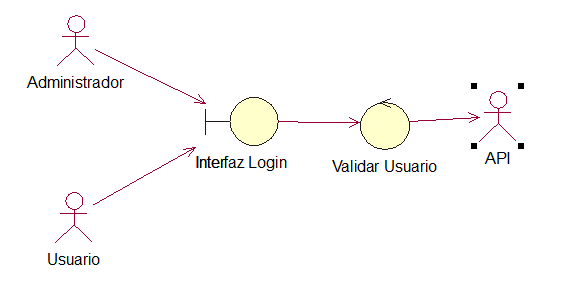
\includegraphics[scale=0.45]{Image/Caso de Uso Login.PNG}
\caption{Caso de Uso Login}
\label{fig:Csha3}
\end{figure}

\begin{figure}[h!]
\centering
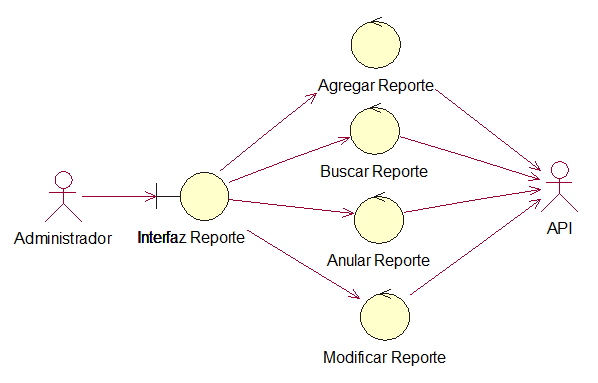
\includegraphics[scale=0.45]{Image/Caso de Uso Reporte.PNG}
\caption{Caso de Uso Reporte}
\label{fig:Csha3}
\end{figure}

\begin{figure}[h!]
\centering
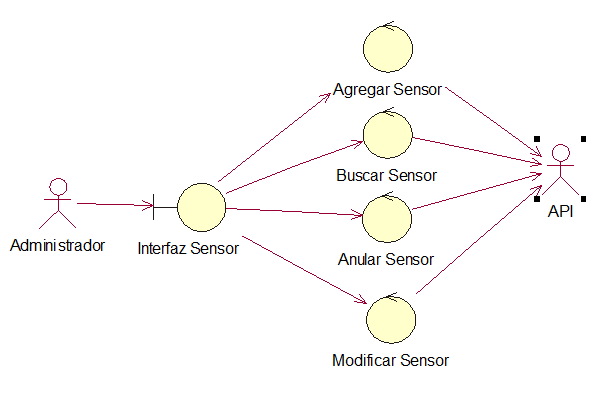
\includegraphics[scale=0.45]{Image/Caso de Uso Sensor.PNG}
\caption{Caso de Uso Sensor}
\label{fig:Csha3}
\end{figure}

\begin{figure}[h!]
\centering
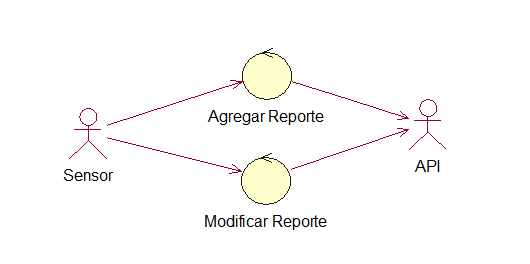
\includegraphics[scale=0.45]{Image/Caso de Uso SensorReporte.PNG}
\caption{Caso de Uso SensorReporte}
\label{fig:Csha3}
\end{figure}

\begin{figure}[h!]
\centering
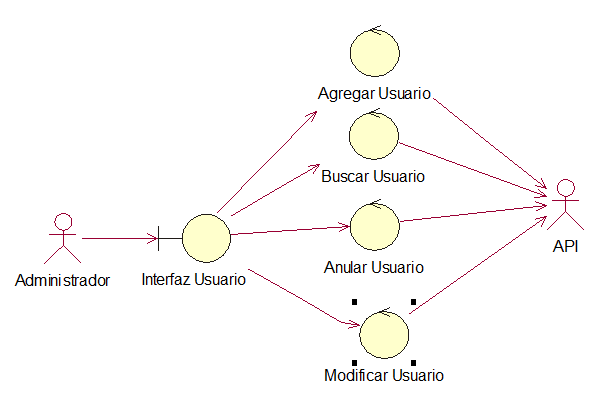
\includegraphics[scale=0.45]{Image/Caso de Uso Usuario.PNG}
\caption{Caso de Uso Usuario}
\label{fig:Csha3}
\end{figure}

\clearpage
\subsection{Diagrama de Arquitectura de la Aplicacion}
Hemos llegado a la conclusion de que eventualmente deberemos usar una API entre el Servidor de base de datos, y esta aplicación.

\begin{figure}[h!]
\centering
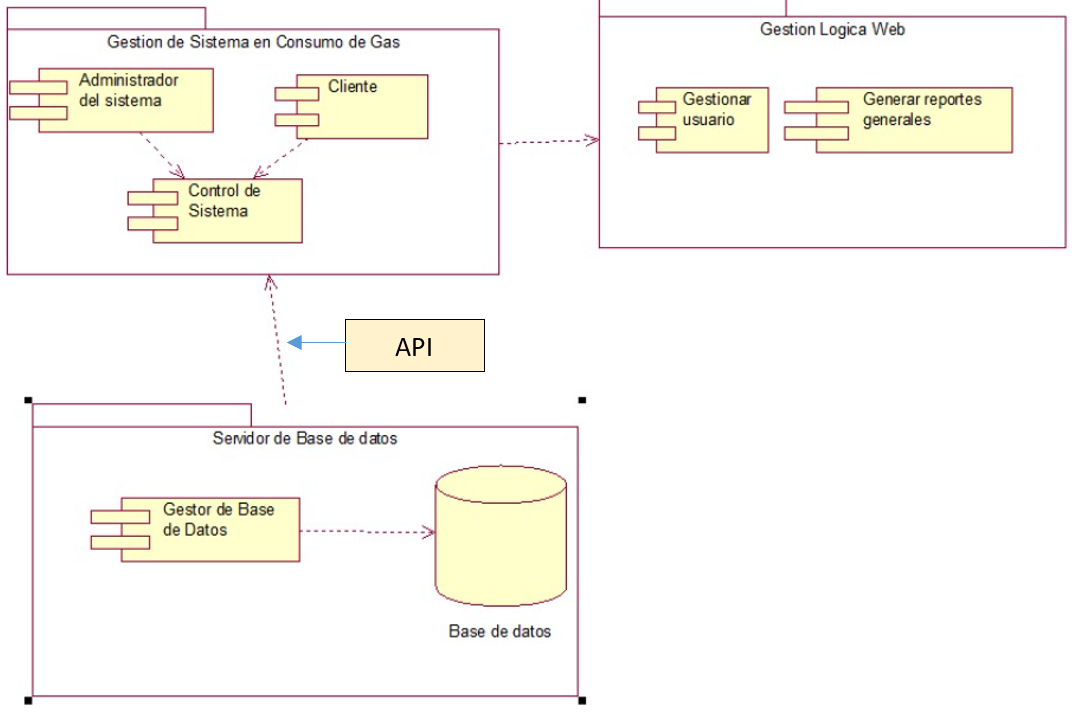
\includegraphics[scale=0.25]{Image/Diagramade Arquitectura.PNG}
\caption{El cambio radicaria en la incorporacion de una API}
\label{fig:Csha3}
\end{figure}

\subsection{Diagrama de Clases de la Aplicacion}
Hay un cambio bastante visible al respecto.

\begin{figure}[h!]
\centering
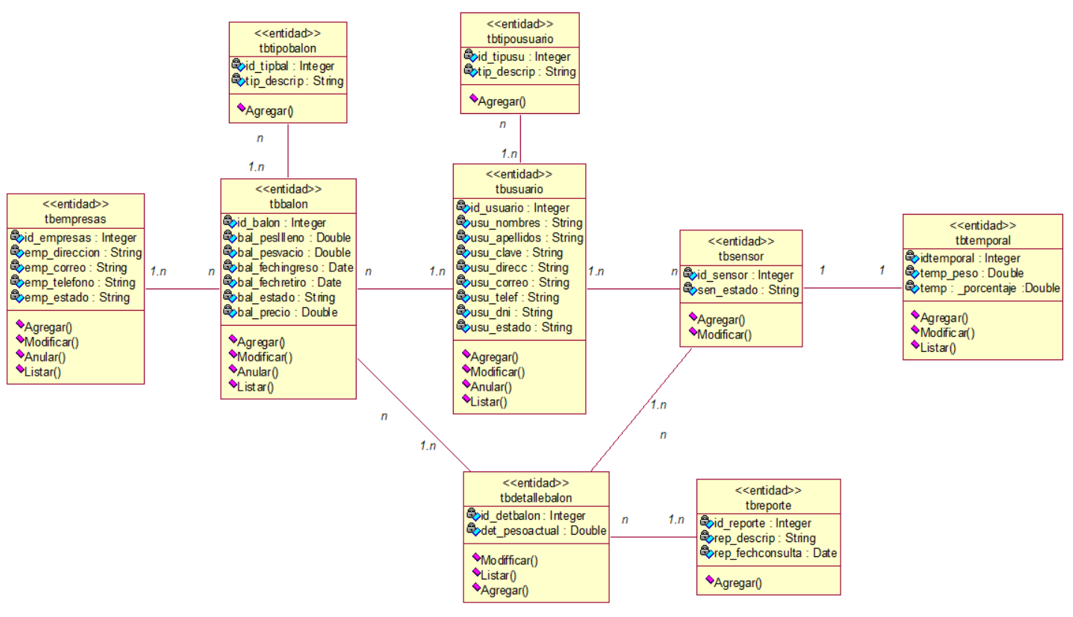
\includegraphics[scale=0.25]{Image/Digrama de clases pre.PNG}
\caption{BD Relacional}
\label{fig:Csha3}
\end{figure}

\begin{figure}[h!]
\centering
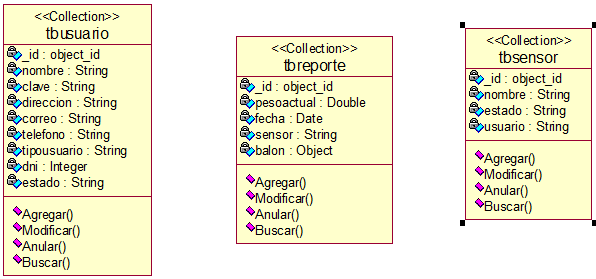
\includegraphics[scale=0.35]{Image/Digrama de clases.PNG}
\caption{BD No Relacional}
\label{fig:Csha3}
\end{figure}

\subsection{Cadena de Conexion y manipulacion en MongoDB}


\begin{figure}[h!]
\centering
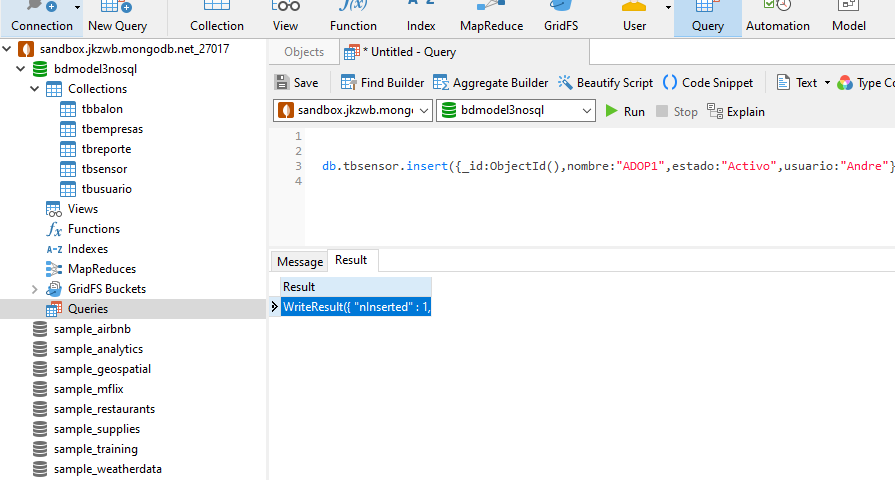
\includegraphics[scale=0.25]{Image/insert.PNG}
\caption{Insert simple}
\label{fig:Csha3}
\end{figure}


\begin{figure}[h!]
\centering
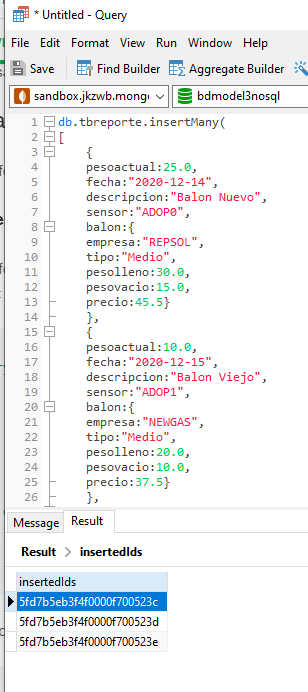
\includegraphics[scale=0.35]{Image/InsertManey.PNG}
\caption{Uso de Insert Many para insertar bastantes documentos a la vez}
\label{fig:Csha3}
\end{figure}

\begin{figure}[h!]
\centering
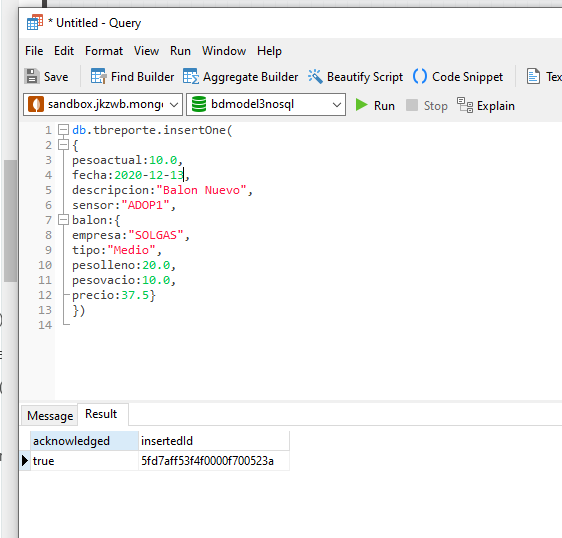
\includegraphics[scale=0.35]{Image/insertOneReporte.PNG}
\caption{Uso de Insert One, que solo permite insertar 1 documento}
\label{fig:Csha3}
\end{figure}

\begin{figure}[h!]
\centering
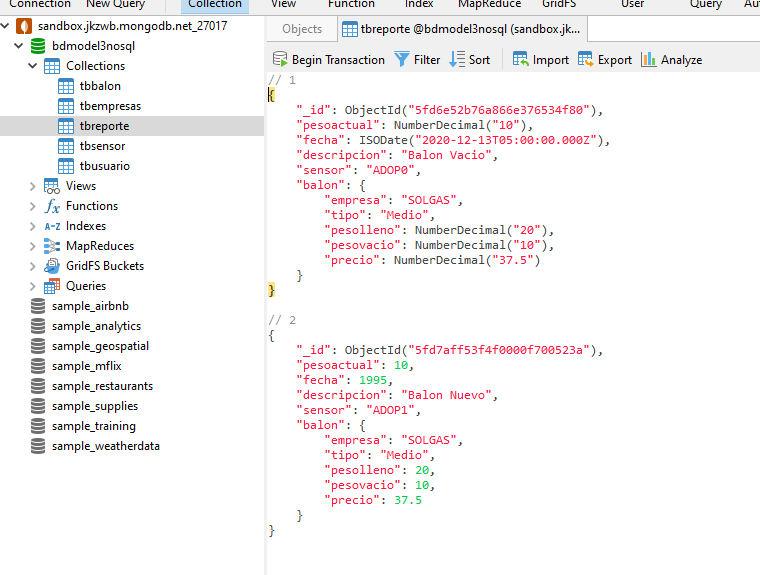
\includegraphics[scale=0.35]{Image/insertOneReporteEfectivo.PNG}
\caption{Un insert de reporte}
\label{fig:Csha3}
\end{figure}

\begin{figure}[h!]
\centering
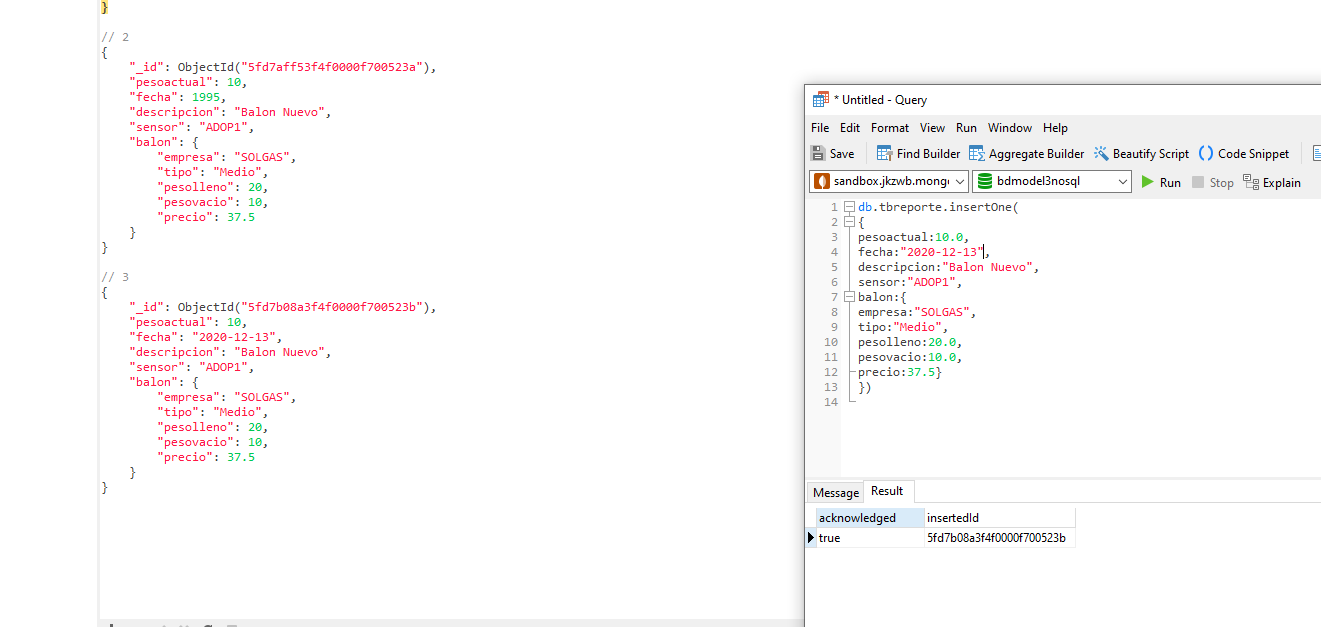
\includegraphics[scale=0.20]{Image/insertOneReporteEfectivoConBuenaFecha.PNG}
\caption{Un insert efectivo con la fecha escrita adecuadamente}
\label{fig:Csha3}
\end{figure}

\begin{figure}[h!]
\centering
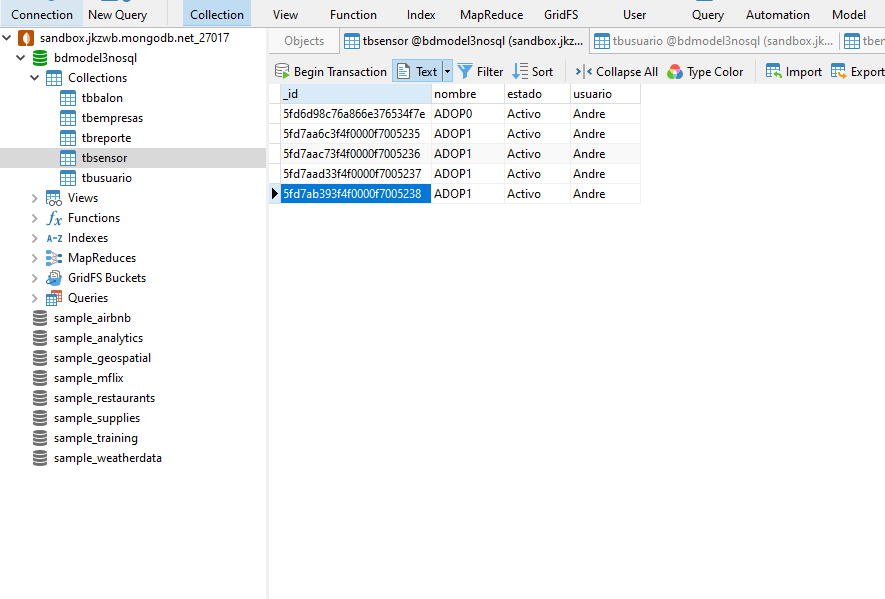
\includegraphics[scale=0.30]{Image/Listado de Sensore.PNG}
\caption{Un listado de los documentos en la coleccion Sensor}
\label{fig:Csha3}
\end{figure}

\begin{figure}[h!]
\centering
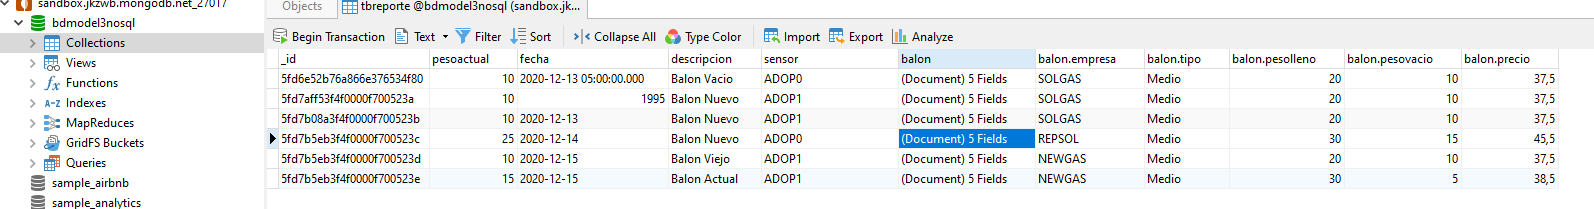
\includegraphics[scale=0.15]{Image/ListReporte.PNG}
\caption{Un listado de los documentos en la coleccion Reporte}
\label{fig:Csha3}
\end{figure}

\begin{figure}[h!]
\centering
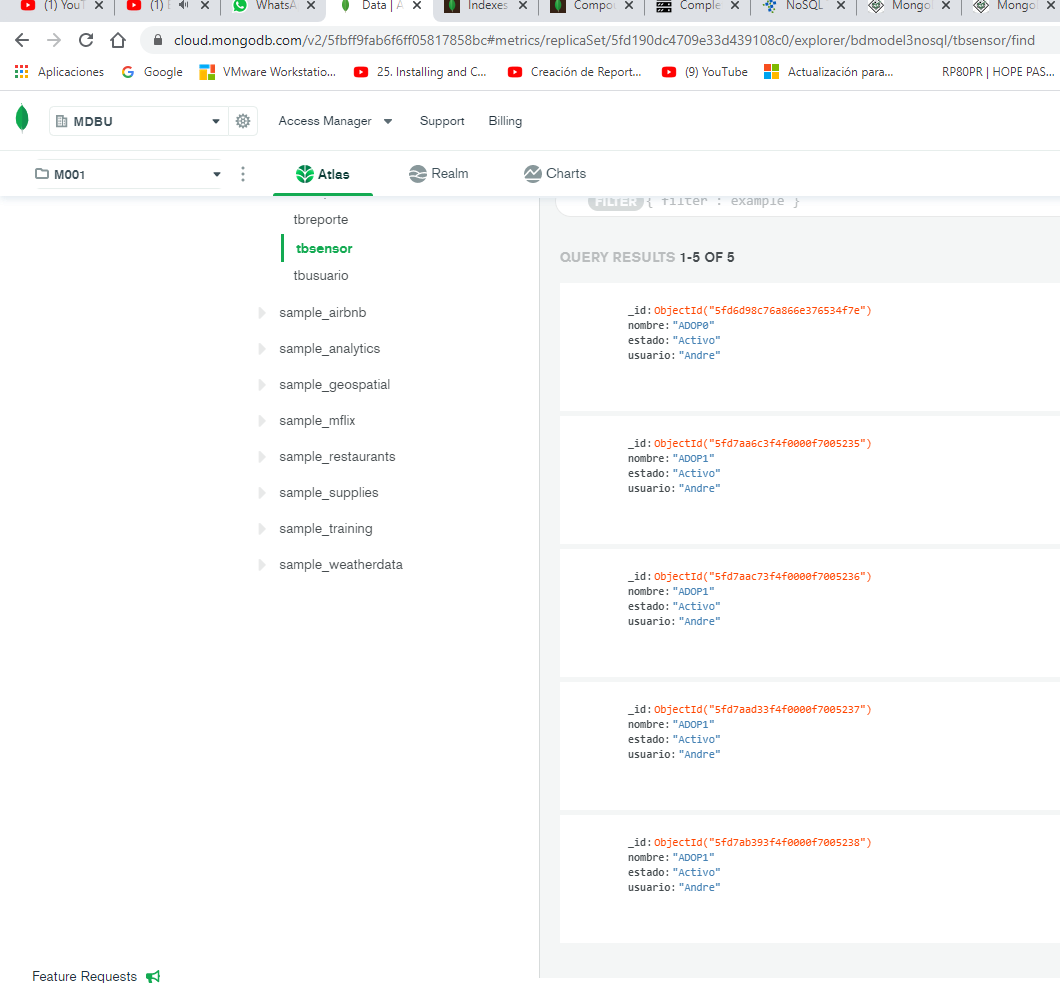
\includegraphics[scale=0.25]{Image/insert,sin que nos demos cuenta.PNG}
\caption{[Se agregaron datos sin que nos dieramos cuenta]}
\label{fig:Csha3}
\end{figure}

\begin{figure}[h!]
\centering
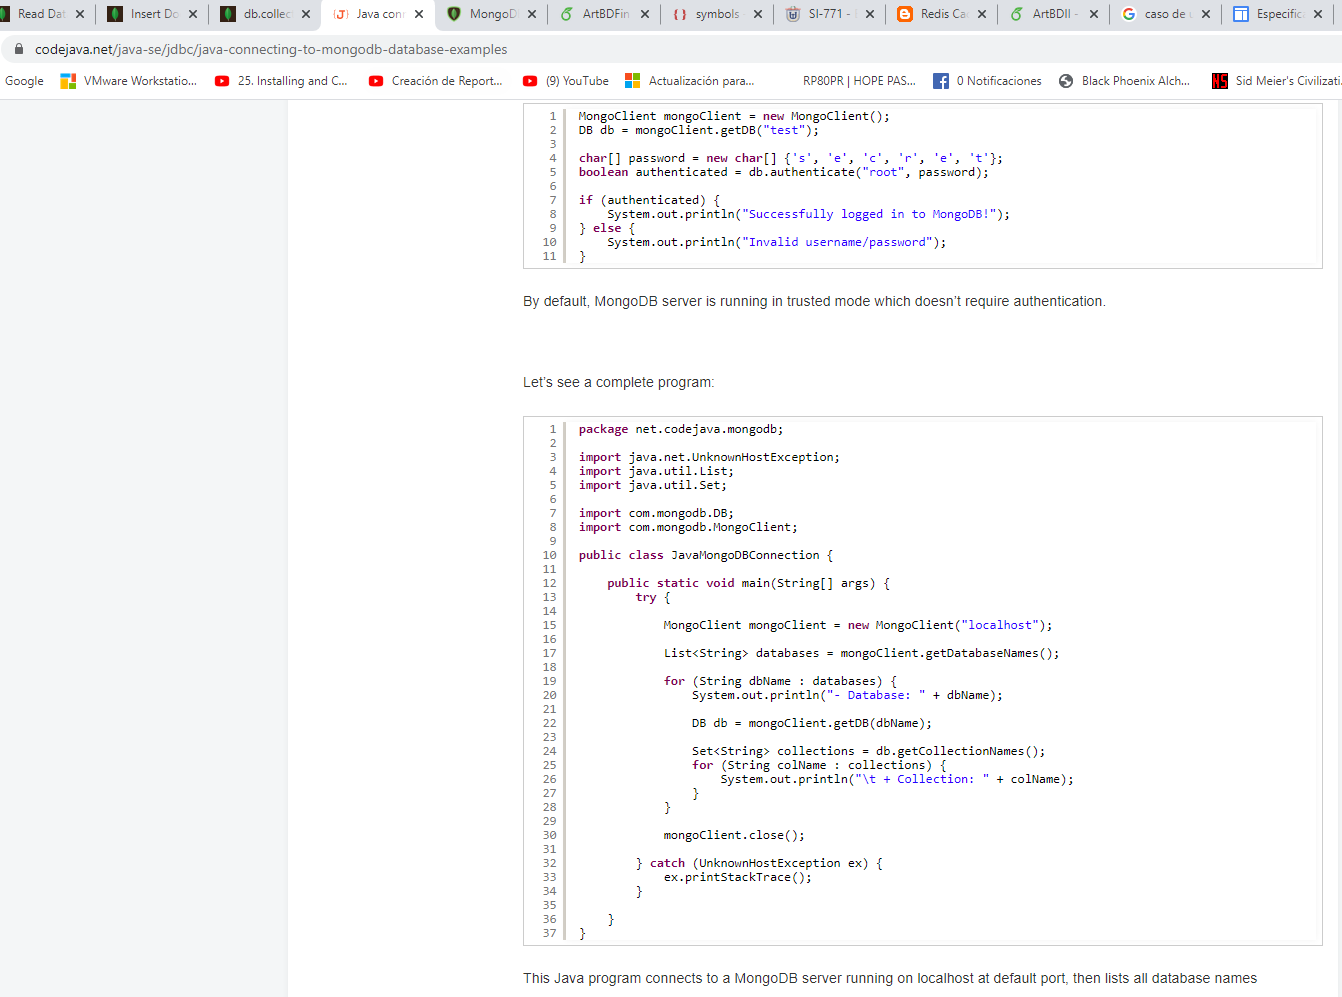
\includegraphics[scale=0.20]{Image/String.PNG}
\caption{Cadena de Conexion de Mongo en Java}
\label{fig:Csha3}
\end{figure}

\clearpage

\subsection{Diccionario de Datos}

\begin{figure}[h!]
\centering
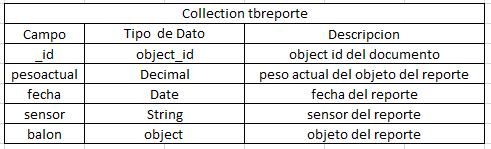
\includegraphics[scale=0.50]{Image/Collection tbreporte.PNG}
\caption{Collection tbreporte}
\label{fig:Csha3}
\end{figure}

\begin{figure}[h!]
\centering
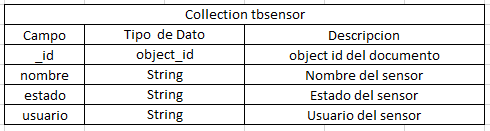
\includegraphics[scale=0.50]{Image/Collection tbsensor.PNG}
\caption{Collection tbsensor}
\label{fig:Csha3}
\end{figure}

\begin{figure}[h!]
\centering
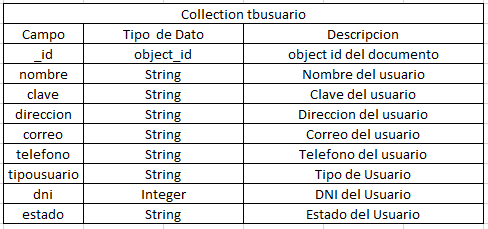
\includegraphics[scale=0.50]{Image/Collection tbusuario.PNG}
\caption{Collection tbusuario}
\label{fig:Csha3}
\end{figure}


\section{Conclusiones}
Hay bastante que mejorar y aplicar.

\section{Recomendaciones}
Se recomienda tener conocimientos previos de SonarQube para revisar las diferentes propuestas a desarrollar para entender de manera fácil y sencilla los posibles errores a la hora de su ejecución.

\section{Bibliográfia}
\item Autor: Juan Sebastián Robayo Colorado, Juan Felipe Talero Gómez(2019).
\newline
\newline
Titulo: Diseño de una herramienta digital para la fiscalización mensual de datos de pozos de petróleo y gas en tiempo real bajo las formas ministeriales de reporte de producción de hidrocarburos
\newline
\newline
Recuperado: http://repositorio.ug.edu.ec/handle/redug/3945
\newline
\newline

\item Autor: Andrea Gabriela Chiriguaya Rodríguez y Víctor Gary Ronquillo Suárez(2019).
\newline
\newline
Titulo: Prototipo de sensor para medir el nivel de gas en una bombona de butano con notificación mediante aplicación android.
\newline
\newline
Recuperado: http://repositorio.ug.edu.ec/handle/redug/3945
\newline
\newline

\item Autor: Muñoz Catalina Morales, Gustavo A , Miramá Víctor F (2020).
\newline
\newline
Titulo: Aplicación de una red de sensores inalámbricos en un ambiente de trabajo industrial.
\newline
\newline
Recuperado: https://www.revistaespacios.com/a20v41n31/a20v41n31p11.pdf
\newline
\newline

\item Autor: Michael Andrés Peña González(2016).
\newline
\newline
Titulo: Diseño e Implementación de Algoritmo para Monitoreo y Control Industrial en Bombas de Gas desde Cabeza de Pozo.
\newline
\newline
Recuperado: http://repository.udistrital.edu.co/bitstream/11349/4747/1/Pec3b1aGonzalezMichaelAndres2016.pdf
\newline
\newline

\end{itemize}
\end{document}